\documentclass[12pt,a4paper]{article}

\usepackage[utf8]{inputenc}

\usepackage[width=200mm,height=280mm,centering]{geometry}

% \usepackage{mathptmx}
\usepackage{palatino}

%\usepackage{chancery}
%\usepackage{antiqua}
%\usepackage{aboensis}
\usepackage{gfsartemisia-euler}
\usepackage[T1]{fontenc}

% \usepackage{fontspec}
% \setmainfont{QTChanceryType}

\usepackage{graphicx}
\usepackage[table]{xcolor}
\usepackage{tikz}
\usetikzlibrary{decorations.text}
\usepackage[hidelinks]{hyperref}

\pagestyle{empty}

%\newcommand{\logo}{\makebox[56mm][c]{\rule{0mm}{66mm}\raisebox{12mm}{
\includegraphics[width=48mm]{logo/aldc-4couleurs-3.pdf}}}}

%\pagecolor{yellow!5}

\usepackage{fontspec}


\begin{document}
\sffamily
\bfseries
%\color{yellow!20}
\parindent=0mm

%%%%%%%%%%%%%% FOND ET LOGOS


\unitlength=1mm
\begin{picture}(0,0)
\fontsize{40pt}{40pt}
\fontspec{QTOKCorral-Ext}
\selectfont
\put(-5,-290){\includegraphics[width=212mm]{../images/Fond-bois-tres-clair-small.jpg}}
\put(15,-270){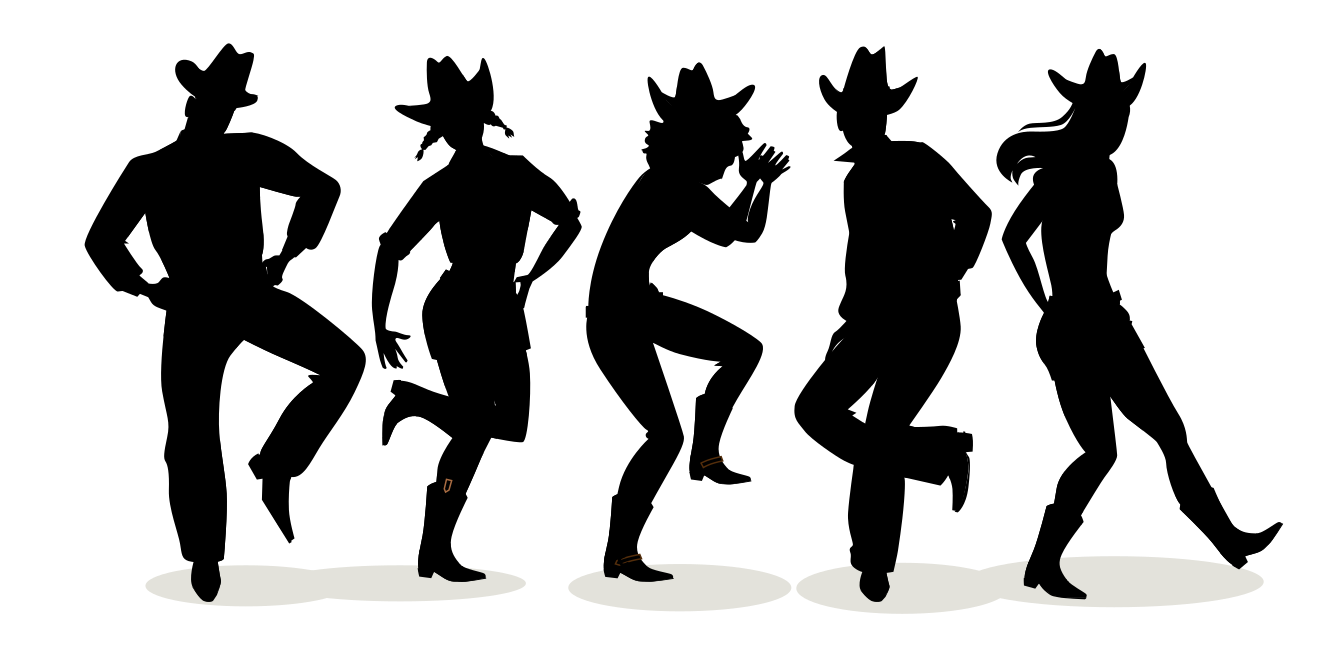
\includegraphics[width=170mm]{../images/groupededanseenligne-ombre.png}}
\put(25,-200){\includegraphics[width=60mm]{../images/barjaud1.png}}
\put(120,-200){\includegraphics[width=60mm]{../images/arreou1.png}}
\put(155,-30){\href{https://alevisdanse.github.io}{
\includegraphics[height=40mm]{../static/images/logo-aldc-contour-noir.pdf}}}
\put(0,-40){\href{https://country-rn10-13.webself.net/}{\includegraphics[height=50mm]{../images/LOGO RN10 officiel-fi36141364x430.png}}}
\put(52,-120){Workshops et mini-bal}
\put(78,-135){animés par}
\end{picture}


%%%%%%%%%%%%%%%%% DATE

\begin{center}
\fontsize{32pt}{36pt}\selectfont
Dimanche \\
6 Décembre 2026\\
\fontsize{20pt}{24pt}\selectfont
  de 14h à 19h
\end{center}



\vspace*{-15mm}



%%%%%%%%%%%%%%%%%%%%% BAL COUNTRY
\begin{center}
\fontspec{QTOKCorral-Ext}
\fontsize{80pt}{80pt}\selectfont
\begin{tikzpicture}
\node (a) at (0,2){};
\node (b) at (18,2){};
\node (c) at (0,0){};
\node (d) at (18,0){};
\node (aa) at (0.15,1.85){};
\node (bb) at (18.15,1.85){};
\node (cc) at (0.15,-0.15){};
\node (dd) at (18.15,-0.15){};
\draw[draw=none, postaction={decorate,decoration={text along path,text align=center,text color=yellow!20,text={STAGE COUNTRY}}}] (aa) to [bend right=-10]  (bb);
\draw[draw=none, postaction={decorate,decoration={text along path,text align=center,text color=yellow!20,text={CATALAN STYLE}}}] (cc) to [bend right=10]  (dd);
\draw[draw=none, postaction={decorate,decoration={text along path,text align=center,text={STAGE COUNTRY}}}] (a) to [bend right=-10]  (b);
\draw[draw=none, postaction={decorate,decoration={text along path,text align=center,text={CATALAN STYLE}}}] (c) to [bend right=10]  (d);
\fontsize{40pt}{40pt}
\selectfont
% \node (e) at (0.5,-8){};
% \node (f) at (5,-3){};
% \node (g) at (9.6,-9.3){};
% \node (h) at (16,-12){};
\draw[draw=none,postaction={decorate,decoration={text along path,text align=center,text={Virginie Barjaud}}}]
  (1.5,-8.5) arc (195:75:3.2);
\draw[draw=none,postaction={decorate,decoration={text along path,text align=center,text={Chrystel Arréou}}}]
  (13.2,-4.6) arc (105:-30:3.2);
\end{tikzpicture}
\end{center}


\vspace*{-120mm}
\vfill

%%%%%%%%%%%%%%%%%%%%% Workshop
\begin{flushleft}
\fontsize{54pt}{54pt}
\fontspec{QTOKCorral-Ext}
\selectfont
%~ Workshops Isabelle Dréau et Chrystel Arréou
\end{flushleft}

%%%%%%%%%%%%%%%%%%%%%

\vspace*{60mm}
\vfill

\begin{minipage}[b]{0.48\linewidth}
\fontsize{20pt}{20pt}\selectfont
Renseignements: \\
\href{mailto:alevisdanse@gmail.com?subject=Stage Catalan 6 decembre}{\texttt{\color{blue!50!black}alevisdanse@gmail.com}} \\
ou\\
\href{mailto:countryrn10@free.fr?subject=Stage Catalan 6 decembre}{\texttt{\color{blue!50!black}countryrn10@free.fr}}\\
~\\
Réservation obligatoire: \\
\includegraphics[height=28mm]{ALDC26-qr.png}
\raisebox{15mm}{\href{https://tinyurl.com/ALDC26}{\texttt{\color{blue!50!black}https://tinyurl.com/ALDC26}}}
\end{minipage}\hfill\begin{minipage}[b]{0.5\linewidth}
\fontsize{20pt}{20pt}\selectfont
\begin{flushright}
Salle Polyvalente de \\
Lévis-Saint-Nom\\
{\fontsize{14pt}{16pt}\selectfont
  (78320, 8 Route d'Yvette)}\\
~\\
    Ouverture des portes: 13h30\\
    ~\\
    Entrée: 10 euros \\
    ~\\
    Buvette et petite \\
    restauration sur place
  \end{flushright}
\end{minipage}

% {\fontsize{14pt}{16pt}\selectfont
% Nous sommes aussi sur FB: \raisebox{-8.5mm}{\includegraphics[width=20mm]{images/fb-aldc-qr-code.jpg}}}

\end{document}

\newpage

\begin{center}
Programme
\end{center}

\begin{description}
\item[13h30] Ouverture des portes
\item[14h] Ouverture du bal playlist CD
\item[15h] Workshop par Chrystel Arréou niveau débutant
\item[16h] Reprise de la playlist
\item[17h] Workshop par Chrystel Arréou niveau novice
\item[18h] Reprise de la playlist
\item[18h30] Apéro offert, pause restauration
\item[20h] Concert Charlie Gon
\item[22h] Reprise de la playlist
\end{description}

\vfill

\begin{center}
Bulletin d'inscription
\end{center}

à envoyer à alevisdanse@gmail.com

Nom, prénom

Club

reservation du repas (boisson + sandwich)

\begin{itemize}
\item sandwich jambon beurre cornichon
\item sandwich fromage
\end{itemize}

\end{document}



% Local variables:
% mode: latex
% TeX-master: t
% TeX-PDF-mode: t
% TeX-engine: luatex
% mode: flyspell
% ispell-local-dictionary: "francais"
% End:
